\documentclass{article}
\usepackage{graphicx} % Required for inserting images
\usepackage[utf8]{inputenc}
\usepackage{polski}
\usepackage[dvipsnames]{xcolor}
\usepackage{indentfirst}
\usepackage{multicol}
\usepackage{geometry}
\usepackage{titlesec}
\usepackage[colorlinks=true, linkcolor=gray, urlcolor=blue, citecolor=green]{hyperref}
\usepackage{makecell}
\usepackage{float}
\usepackage[polish]{babel}
\usepackage[T1]{fontenc}
\usepackage[justification=centering]{caption}
\usepackage[utf8]{inputenc} 
\usepackage{subfig}
\usepackage{changepage}


\usepackage{mwe} % for 'example-image'
\usepackage{newfloat}
\DeclareFloatingEnvironment{graph}
\addto\captionspolish{%
  \renewcommand{\graphname}{Wykres}%
  \renewcommand{\figurename}{Zdjęcie}%
  \renewcommand{\tablename}{Tabela}%
}


\begin{document}

\begin{titlepage}
    \begin{center}
        \vspace*{1cm}
            
        \Huge
        \textbf{Sprawozdanie z laboratorium 3}
            
        \vspace{0.5cm}
        \LARGE
        Modbus 
            
        \vspace{1.5cm}
            
        \textbf{Łukasz Janusz\\Marek Generowicz}

        \normalsize      
        \textcolor{gray}{27.03.2025}
        \vfill
        \begin{figure}[hb]
            \centering
            
\includegraphics[width=0.5\textwidth]{media/Logo_AGH.jpg}
        \end{figure}   
    \end{center}
\end{titlepage}

\section{Wstęp}

\begin{figure}[H]
    \centering
    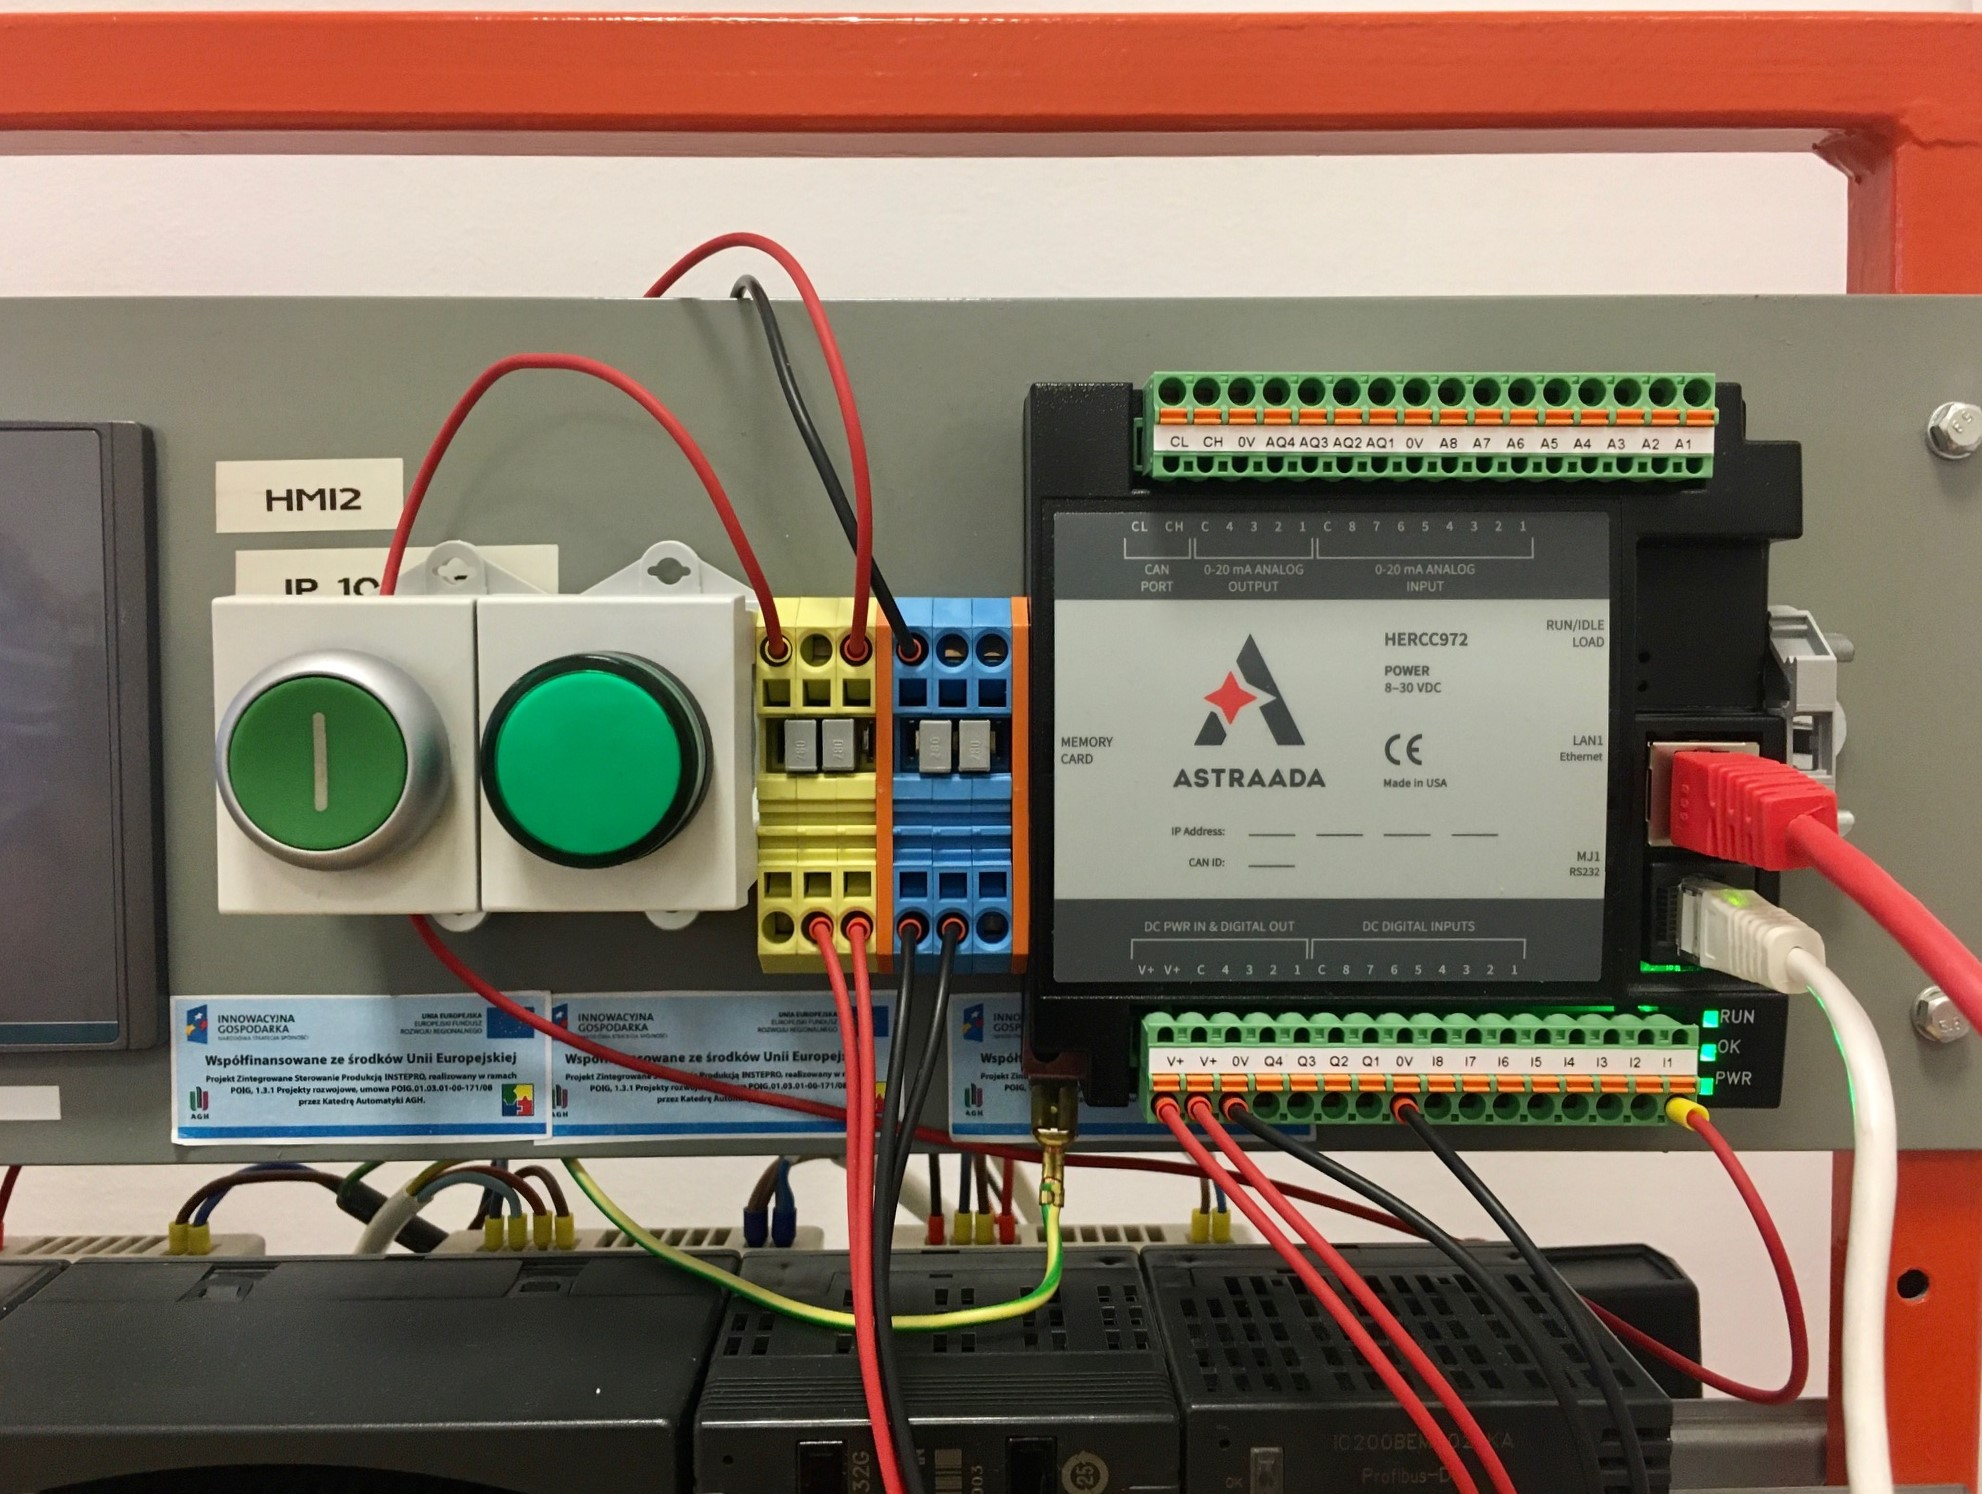
\includegraphics[width=0.92\textwidth]{media/0_stanowisko.jpg}
    \caption{Stanowisko laboratoryjne (zdjęcie z konspektu)}
    \label{fig:stanowisko}
\end{figure}


\newpage
\section{Przygotowanie projektu oraz programu w Cspace}


Przed przystąpieniem do ćwiczeń należało ustawić parametry sieciowe zgodnie z zdjęciem \ref{fig:zdj1} oraz potwierdzić konfiguracje za pomocą ethernetu wraz z podaniem poprawnego adresu IP, dzięki czemu możliwa jest komunikacja z PLC przez ethernet.
\begin{figure}[H]
    \centering
    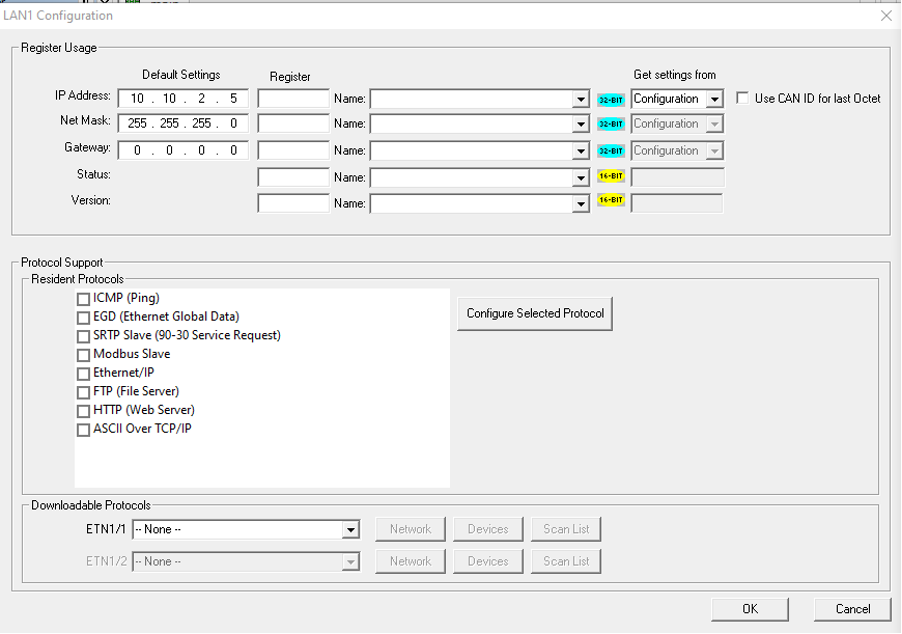
\includegraphics[width=0.5\textwidth]{media/4_0KonfiguracjaLan.png}
    \caption{Ustawienia parametrów LAN1 w Cspace}
    \label{fig:zdj1}
\end{figure}

Dzięki połączeniu z PLC w kolejnych krokach możliwe będzie przesyłanie kodu z komputera do PLC oraz odczyt i zapis danych z rejestrów Modbus. Z powodu że w PLC dalej pamiętany jest kod innej grupy na dole ekranu jednym z parametrów jest \textit{Not Equal}, tak jak na zdjęciu \ref{fig:zdj2}, co oznacza że kod który jest zapisany w PLC nie jest taki sam jak kod zapisany w aplikacji.
\begin{figure}[H]
    \centering
    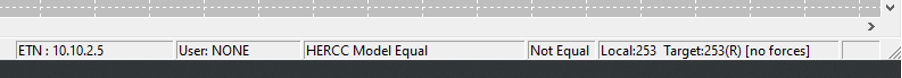
\includegraphics[width=0.5\textwidth]{media/4_1BezKody.png}
    \caption{Listwa statusu z niespójnym kodem w PLC}
    \label{fig:zdj2}
\end{figure}

\newpage
Następnie należało stworzyć prosty układ do zapalania diody kiedy guzik zostanie kliknięty oraz zgaszenia jej kiedy przestanie guzik nie będzie kliknięty. Na zdjęciu \ref{fig:zdj3} w listwie statusu widać również że kod został pomyślnie wgrany i zgadza się z tym co jest w PLC.

\begin{figure}[!ht]
    \centering
        % Pod figura 1
        \subfloat[Kod programu]{    
            \centering
            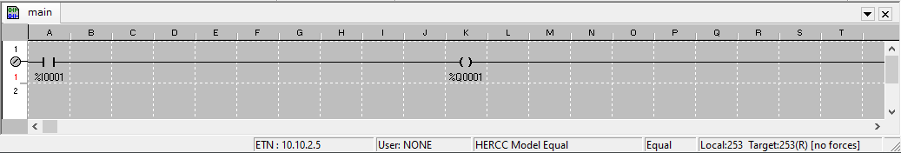
\includegraphics[width=0.5\textwidth]{media/4_2Zkodem.png}
            \label{fig:zdj3}}
        % Pod figura 2
        \subfloat[Debugowanie aktywnego układu]{
            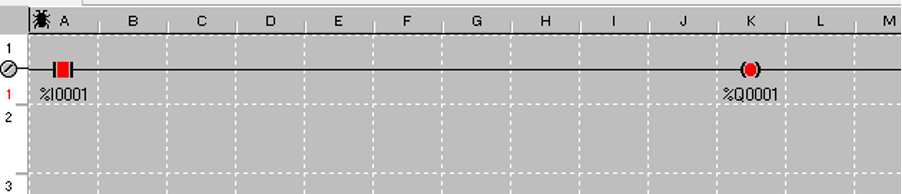
\includegraphics[width=0.5\textwidth]{media/4_3DebugON.png}            \label{fig:zdj4}
        }
   
        \hfill
     % Pod figura 1
    \subfloat[Rzeczywisty układ aktywny]{
        \includegraphics[width=0.5\textwidth]{media/4_5RzeczywistyprzyciskOFF.png}
        \label{fig:zdj5}}
    % Pod figura 2
    \subfloat[Rzeczywisty układ nieaktywny]{
        \includegraphics[width=0.5\textwidth]{media/4_4RzeczywistyprzyciskON.png}
        \label{fig:zdj6}
    }
    \caption{Konfiguracja kanałów modułu}
    \label{fig:main1}
\end{figure}


\newpage
\section{Obsługa oraz testy komunikacji}

\begin{figure}[H]
    \centering
    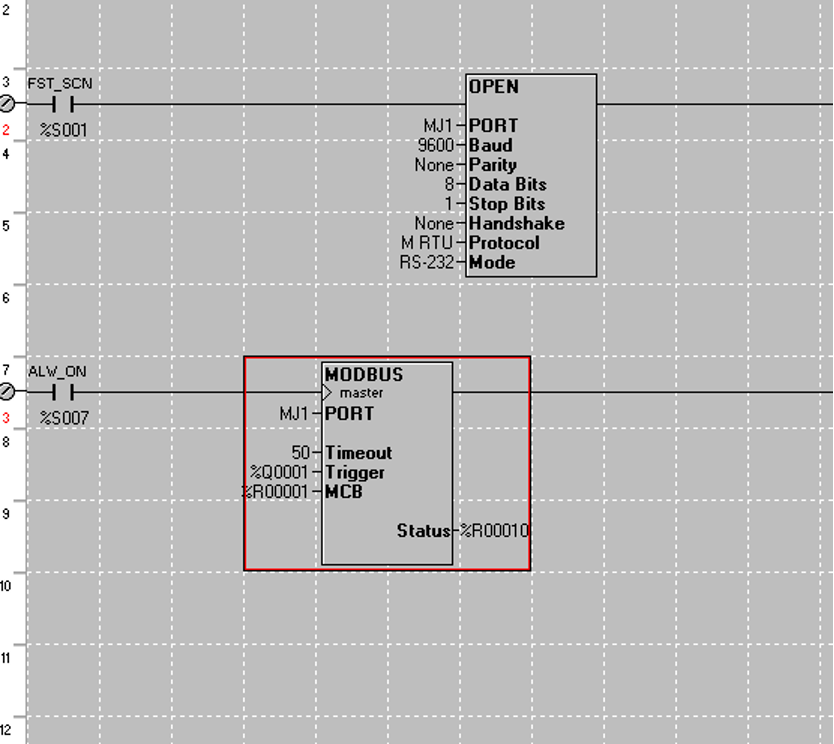
\includegraphics[width=0.5\textwidth]{media/5_1_Kolejnebloczki.png}
    \caption{Stanowisko laboratoryjne (zdjęcie z konspektu)}
    \label{fig:zdj7}
\end{figure}


\begin{figure}[H]
    \centering
    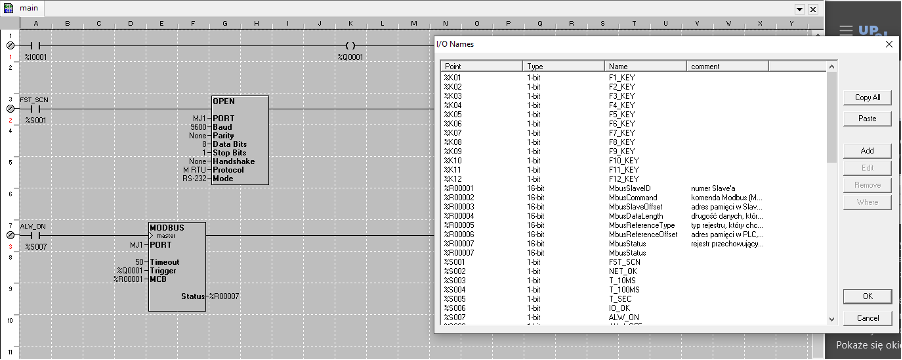
\includegraphics[width=0.5\textwidth]{media/5_2Kod&I:Onames.png}
    \caption{Stanowisko laboratoryjne (zdjęcie z konspektu)}
    \label{fig:zdj8}
\end{figure}


\begin{figure}[H]
    \centering
    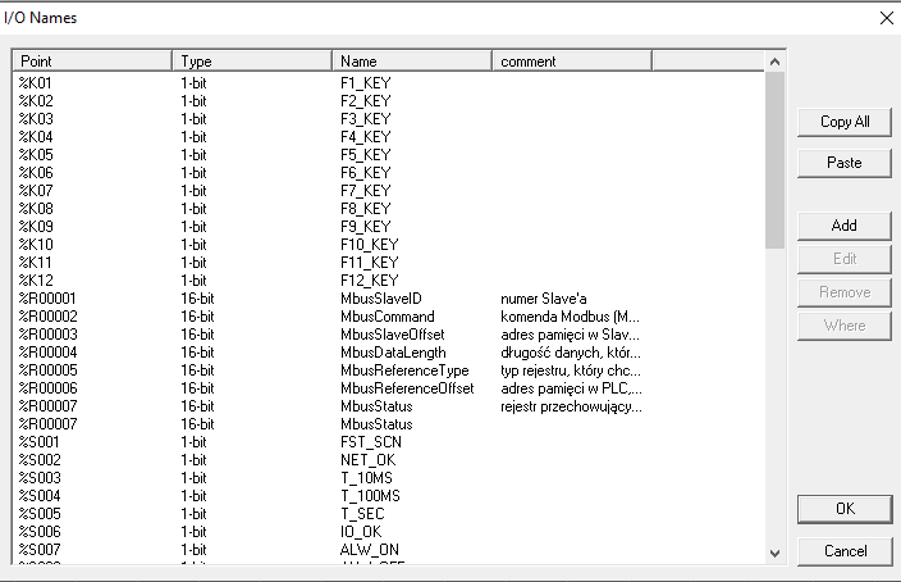
\includegraphics[width=0.5\textwidth]{media/5_3_I:Onames.png}
    \caption{Stanowisko laboratoryjne (zdjęcie z konspektu)}
    \label{fig:zdj9}
\end{figure}


\begin{figure}[H]
    \centering
    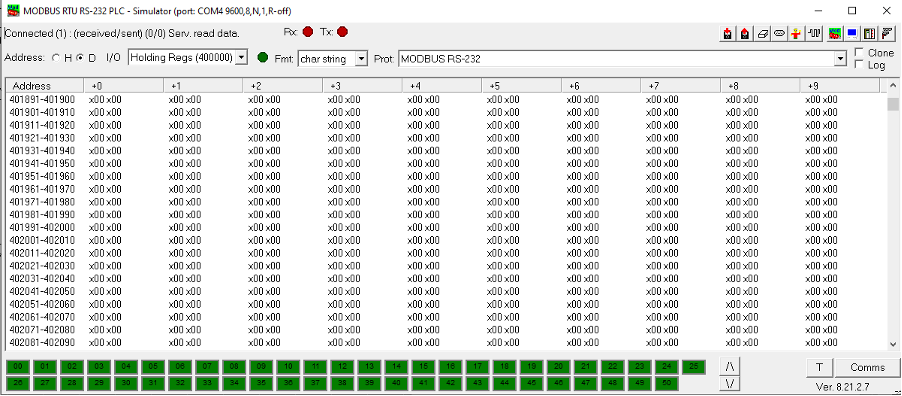
\includegraphics[width=0.5\textwidth]{media/5_4_Modbusapp.png}
    \caption{Stanowisko laboratoryjne (zdjęcie z konspektu)}
    \label{fig:zdj10}
\end{figure}

\subsection{Test 1}


\begin{figure}[H]
    \centering
    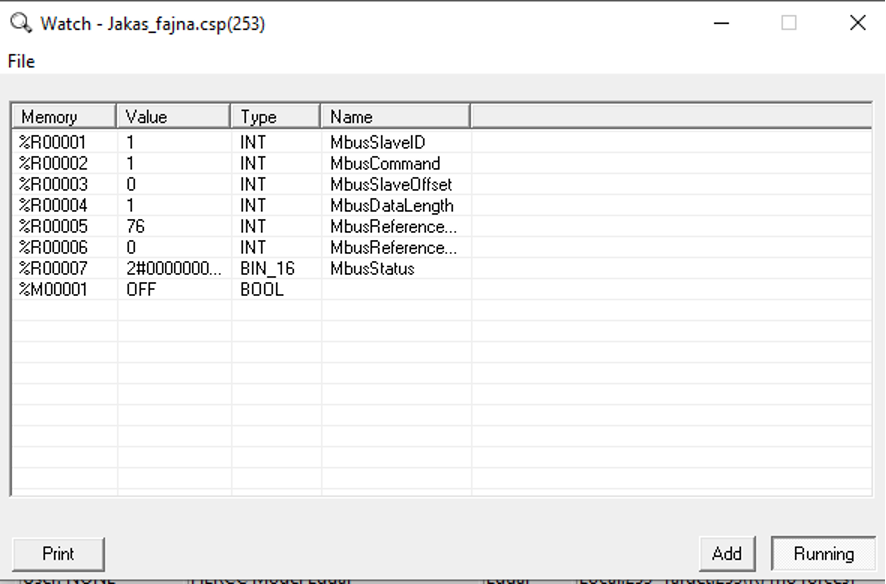
\includegraphics[width=0.5\textwidth]{media/5_test1_1_Watchzmienne.png}
    \caption{Stanowisko laboratoryjne (zdjęcie z konspektu)}
    \label{fig:zdj11}
\end{figure}


\begin{figure}[H]
    \centering
    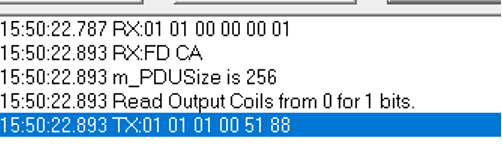
\includegraphics[width=0.5\textwidth]{media/5_test1_2_comszModbusapp.png}
    \caption{Stanowisko laboratoryjne (zdjęcie z konspektu)}
    \label{fig:zdj12}
\end{figure}


\begin{figure}[H]
    \centering
    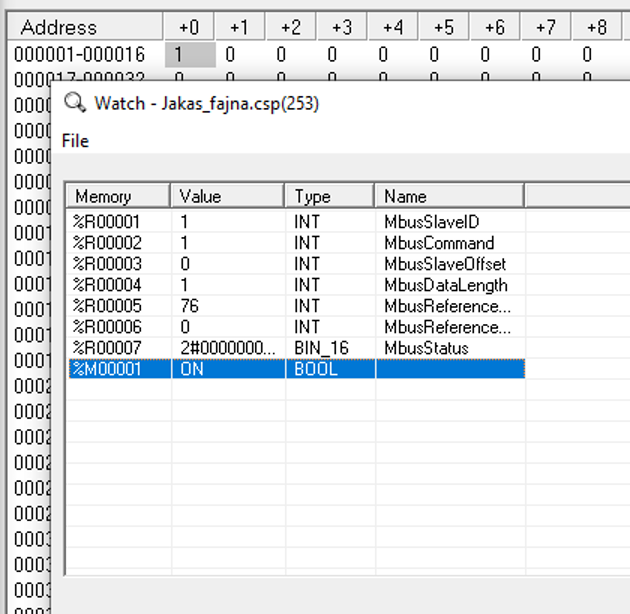
\includegraphics[width=0.5\textwidth]{media/5_test1_3_ONnacewce.png}
    \caption{Stanowisko laboratoryjne (zdjęcie z konspektu)}
    \label{fig:zdj13}
\end{figure}

\subsection{Test 2}


\begin{figure}[H]
    \centering
    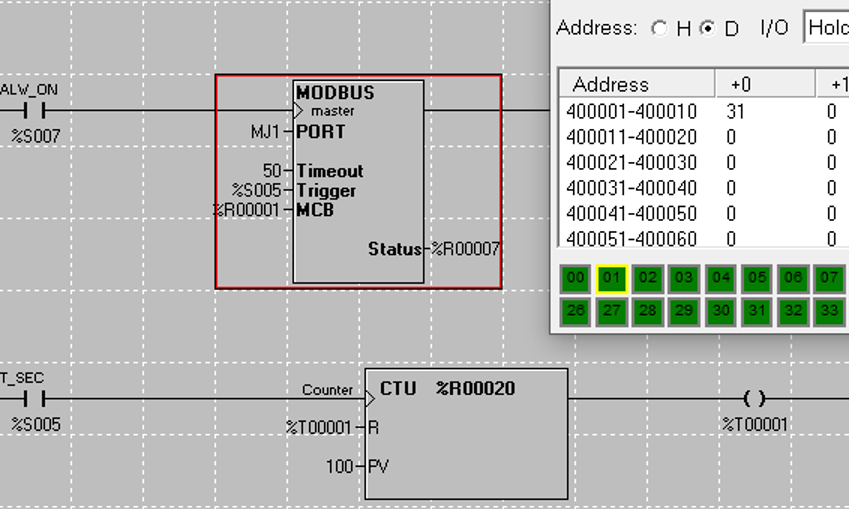
\includegraphics[width=0.5\textwidth]{media/5_test2_1_timer.png}
    \caption{Stanowisko laboratoryjne (zdjęcie z konspektu)}
    \label{fig:zdj14}
\end{figure}


\begin{figure}[H]
    \centering
    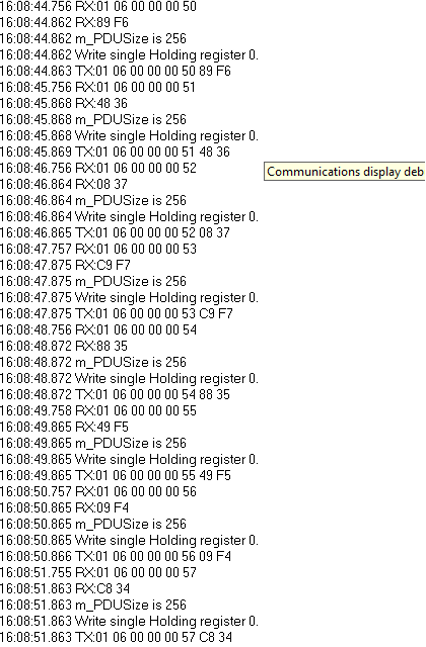
\includegraphics[width=0.5\textwidth]{media/5_test2_2_rejestrzModbusapp.png}
    \caption{Stanowisko laboratoryjne (zdjęcie z konspektu)}
    \label{fig:zdj15}
\end{figure}

\newpage
\section{Zadania}
\subsection{Zadanie 1}

\begin{figure}[H]
    \centering
    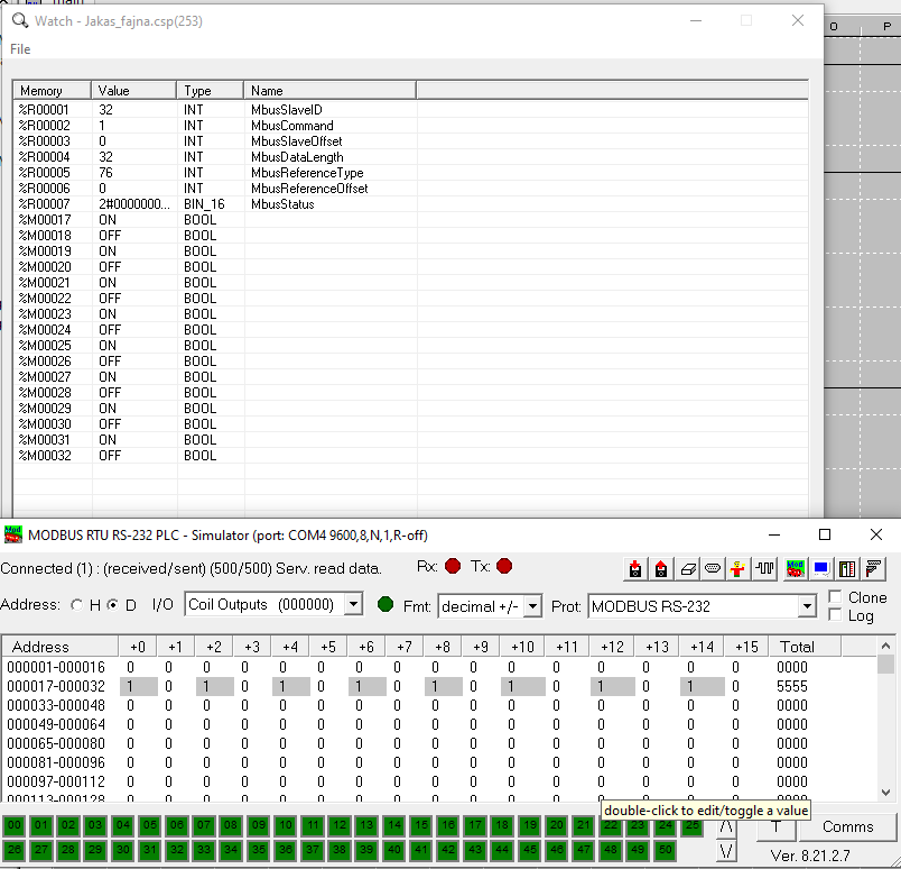
\includegraphics[width=0.5\textwidth]{media/7_1_1_rejestr.png}
    \caption{Stanowisko laboratoryjne (zdjęcie z konspektu)}
    \label{fig:zdj16}
\end{figure}

\begin{figure}[H]
    \centering
    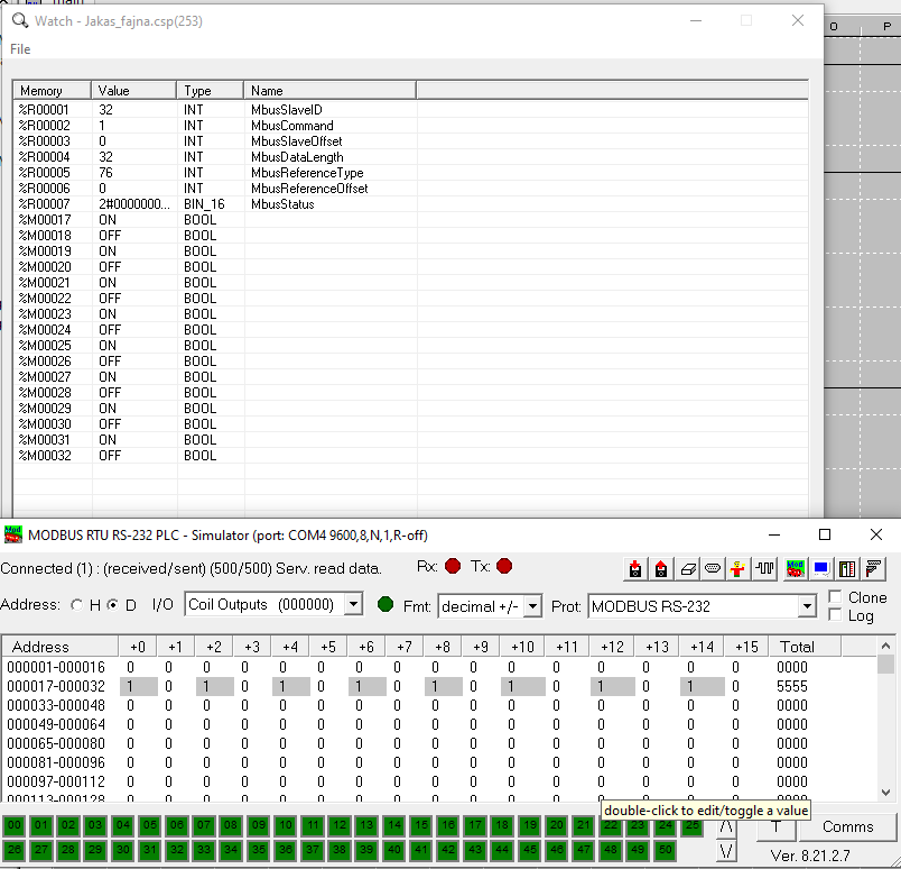
\includegraphics[width=0.5\textwidth]{media/7_1_2_WatchTable.png}
    \caption{Stanowisko laboratoryjne (zdjęcie z konspektu)}
    \label{fig:zdj17}
\end{figure}


\begin{figure}[H]
    \centering
    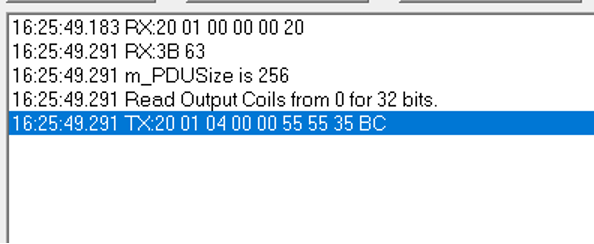
\includegraphics[width=0.5\textwidth]{media/7_1_3_comsy.png}
    \caption{Stanowisko laboratoryjne (zdjęcie z konspektu)}
    \label{fig:zdj18}
\end{figure}

\subsection{Zadanie 2}


\begin{figure}[H]
    \centering
    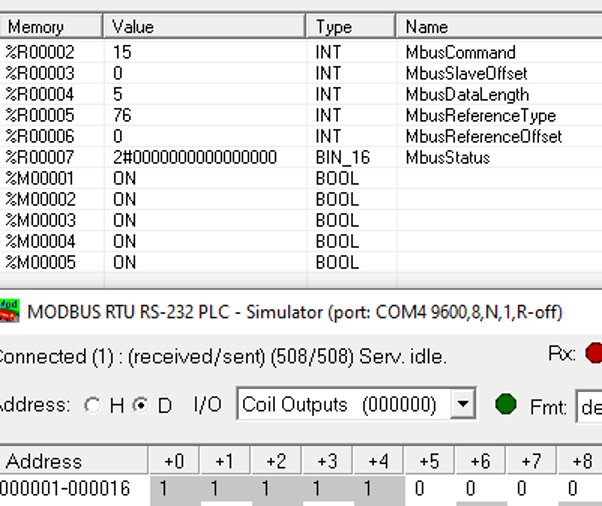
\includegraphics[width=0.5\textwidth]{media/7_2_1_watchtable.png}
    \caption{Stanowisko laboratoryjne (zdjęcie z konspektu)}
    \label{fig:zdj19}
\end{figure}


\begin{figure}[H]
    \centering
    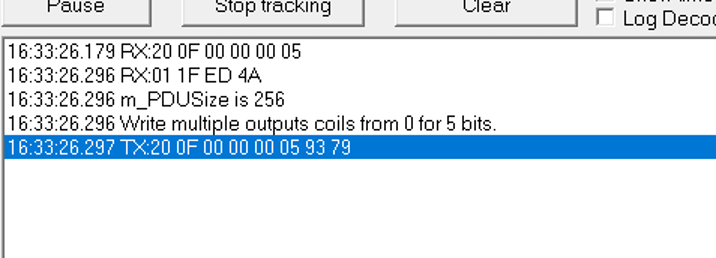
\includegraphics[width=0.5\textwidth]{media/7_2_2_comsy.png}
    \caption{Stanowisko laboratoryjne (zdjęcie z konspektu)}
    \label{fig:zdj20}
\end{figure}


\subsection{Zadanie 3}


\begin{figure}[H]
    \centering
    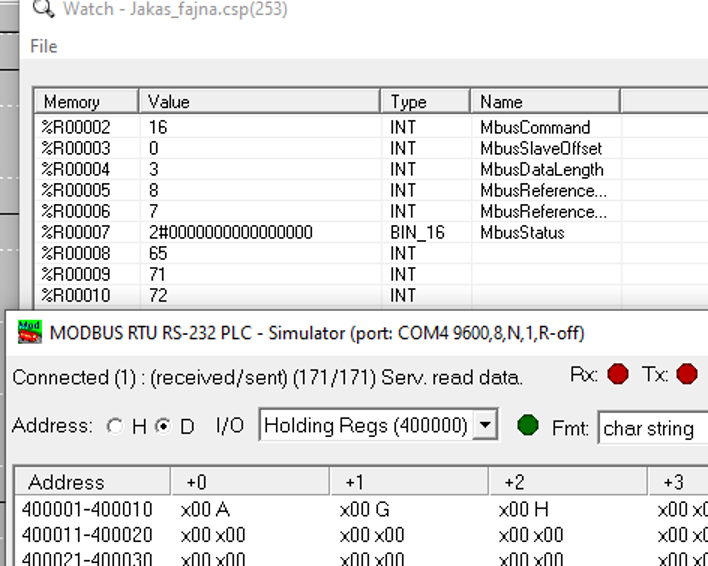
\includegraphics[width=0.5\textwidth]{media/7_3_1_napis.png}
    \caption{Stanowisko laboratoryjne (zdjęcie z konspektu)}
    \label{fig:zdj21}
\end{figure}


\begin{figure}[H]
    \centering
    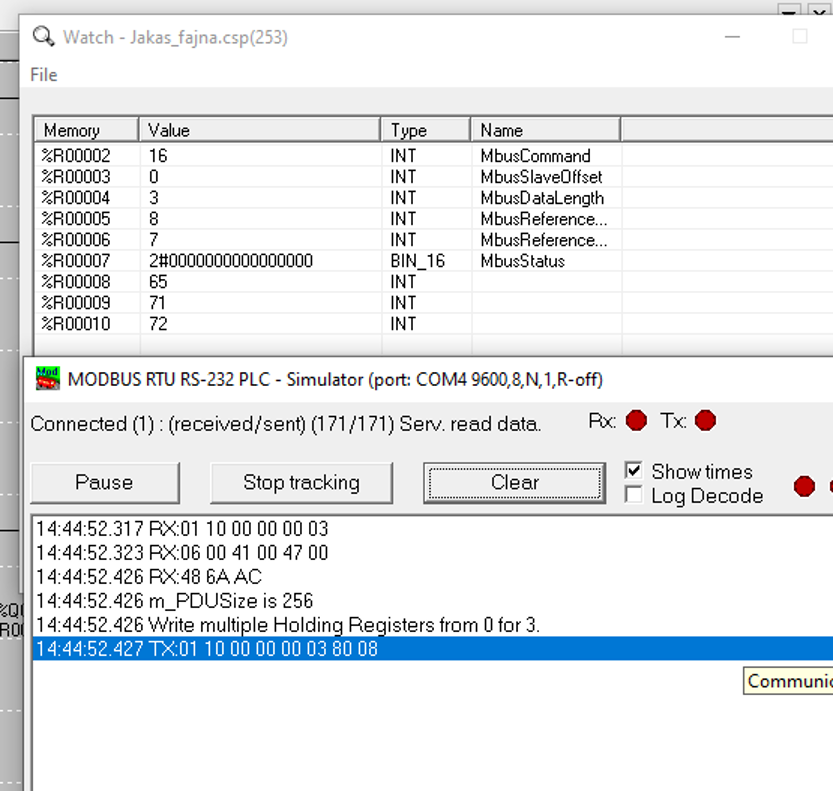
\includegraphics[width=0.5\textwidth]{media/7_3_2_comsy.png}
    \caption{Stanowisko laboratoryjne (zdjęcie z konspektu)}
    \label{fig:zdj22}
\end{figure}


\subsection{Zadanie 4}


\begin{figure}[H]
    \centering
    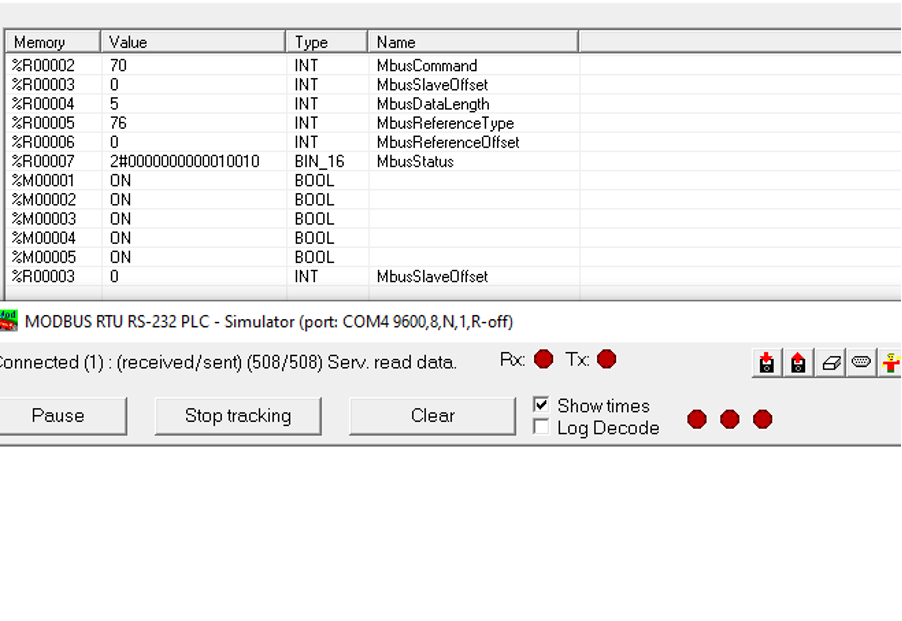
\includegraphics[width=0.5\textwidth]{media/7_4_1_niepoprawnykod.png}
    \caption{Stanowisko laboratoryjne (zdjęcie z konspektu)}
    \label{fig:zdj23}
\end{figure}


\begin{figure}[H]
    \centering
    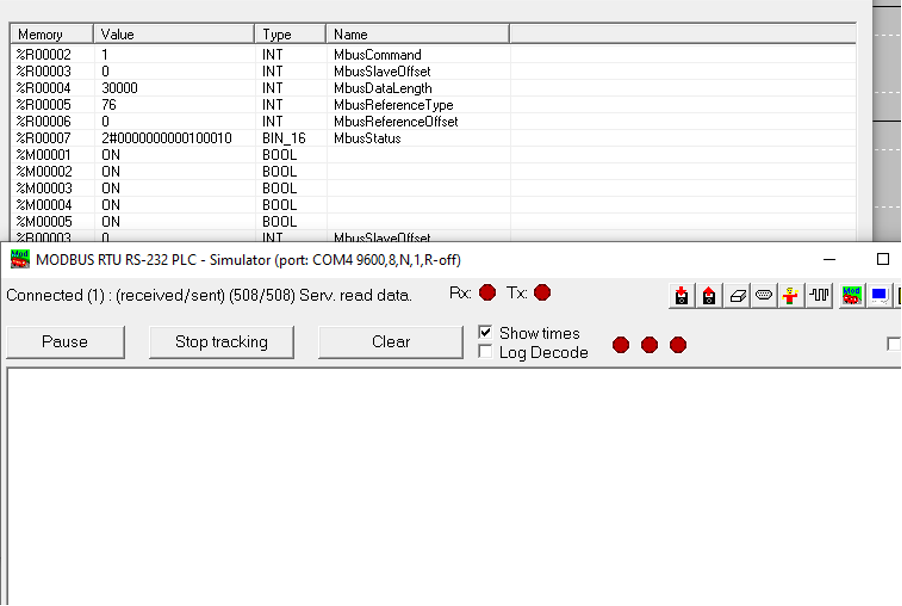
\includegraphics[width=0.5\textwidth]{media/7_4_2_niepoprawnyzakresdanych.png}
    \caption{Stanowisko laboratoryjne (zdjęcie z konspektu)}
    \label{fig:zdj24}
\end{figure}

\end{document}
